\section{Практические аспекты использования систем условных эффектов}

\subsection{Извлечение информации из схем эффектов}

\label{section-info-gathering}

\subsubsection{Два направления вывода информации}

По итогам прошлой главы, мы научились получать схему эффектов для произвольного вызова (при условии, конечно, что все участвующие в нем функции аннотированы схемами). Теперь мы хотели бы научиться извлекать из полученных схем полезную информацию.

В целом, мы можем попытаться извлечь информацию из схемы с помощью двух различных подходов:

\begin{itemize}
    \item Зная некоторую информацию о контексте исполнения, попытаться понять, какие посылки исполняются и какие эффекты может иметь вычисление. Мы будем называть этот подход \term{прямым направлением вывода}, т.к. он сонаправлен с потоком вычислений в программе.

    \item Зная, что подпрограмма сгенерировала некоторые эффекты, попытаться понять, какой вид имел контекст исполнения. Мы будем называть этот подход \term{обратным направлением вывода}, т.к. он противонаправлен потоку вычислений в программе.

\end{itemize}

Рассмотрим для примера следующую схему:

\schema{assertIsNull(x)}
{
    \es{x == null} $\rightarrow$ \es{Returns Unit} \\
    \es{x != null} $\rightarrow$ \es{Throws AssertionError}
}{}

Тогда мы можем извлечь некоторую пользу из этой схемы двумя способами, соответствующими описанным выше подходами:

\begin{itemize}
    \item Понять, что пользователь передает в эту функцию переменную, которая гарантированно не является \code{null}, и предупредить о том, что это действие наверняка вызовет исключение. Как следствие, весь последующий код в данном блоке является недостижимым, о чем также можно сообщить, если это поддерживается инструментами разработки:

    \begin{minted}{kotlin}
        ...
        assertIsNull("Constant string can not be null")
        println("This statement is unreachable!")
        ...
    \end{minted}

    \item Мы можем зайти и с другого конца. Можно посмотреть на следующее после вызова выражение и понять, что вычисление может дойти до него только если исключение не было сгенерировано, т.е. если аргумент, переданный в \code{assertIsNull}, не является \code{null}

    \begin{minted}{kotlin}
        val s: String?
        ... <initialize s> ...

        assertIsNull(s)
        println(s.length)  // here we can be sure that 's != null'
    \end{minted}

    Также как и в предыдущем примере, для того, чтобы конечный пользователь ощутил реальную пользу от этого анализа, необходимо, чтобы инструмент поддерживал некоторый механизм, для которого такая информация была бы полезна. Для этого подхода отлично подходит механизм умных приведений типа в \lang{Kotlin} -- с его помощью мы можем автоматически уточнить тип переменной \code{s} из последнего примера.
\end{itemize}

Алгоритм для прямого вывода достаточно прост и интуитивен -- нужно просто вычислить все операторы в данном контексте, и затем аккуратно собрать эффекты. Некоторые нетривиальности могут возникнуть при обработке посылок, которые оказались вычисленными не до конца, т.е. когда имеющейся в распоряжении информации о контексте не хватает для того, чтобы сделать вывод о том, верна эта посылка или же нет. Однако в таком случае сложно предложить какой-то общий подход к разрешению подобных ситуаций, поскольку это тесно связано с понятием консервативного приближения, и, как следствие, конкретного типа анализа.

В связи с этим, мы не будем заострять внимание на прямом выводе, а вместо этого подробнее рассмотрим алгоритм обратного вывода ниже.


\subsubsection{Алгоритм обратного вывода}

\label{section-back-inference}

Алгоритм обратного вывода состоит из нескольких подчастей:

\begin{enumerate}
    \item Операция \term{фильтрации}, который оставляет в схеме только интересные нам выражения. Например, если мы хотим узнать вид контекста при условии, что функция успешно завершилась, то этому алгоритму будет передано выражение \code{Returns ???}, и он вернет только те утверждения, которые имеют в заключении эффект \code{Returns}.

    \item Операция \term{слияния}, который принимает на вход набор утверждений, полученных после фильтрации, и объединяет информацию, заложенную в этих утверждениях.
\end{enumerate}

Начнем с алгоритма фильтрации. Для того, чтобы понять, как он устроен, опишем более формально то, что он должен делать:

\begin{definition}
    Пусть дано выражение $q$ и утверждение $s$. Будем говорить, что $q$ \term{влечет} $s$ ($s$ \term{следует из} $q$), если информации о том, что были сгенерированы эффекты из заключения $s$ достаточно для того, чтобы сделать вывод, что  имел место эффект $q$. Далее мы будем говорить, что $s_{effects}$ влечет $q$ ($q$ следует из $s_{effects}$)
\end{definition}

Поясним это примером. Рассмотрим схему:

\schema{A}
{
    \es{x is String} $\rightarrow$ \es{Returns(true)} \\
    \es{y != null} $\rightarrow$ \es{Calls(f, 1)}
}{}

Рассмотрим первое утверждение из схемы. Оно, очевидно, следует из выражения \code{Returns true}. Но что более интересно, оно следует также и из выражения \code{Returns ???} -- действительно, если заключение утверждения верно (т.е. функция вернула \code{true}), то, конечно, верно, что функция завершилась (т.е. буквально \code{Returns ???})



Теперь, вооружившись отношением <<влечет>> и дуальным к нему <<следует>>, мы можем описать суть алгоритма фильтрации:

\begin{definition}
    \term{Операция фильтрации} схемы $S$ по выражению $q$ выдает схему $S'$ состоящую только из таких утверждений $S$, которые следуют из $q$. Будем обозначать эту операцию как $Filter(S, q)$
\end{definition}


\bigskip

Перейдем теперь к операции слияния. Будем считать, что нам дана некоторая схема $S$ вычисления $f$, и необходимо собрать информацию, заложенную в ее утверждениях. Введем понятие \term{приближенного контекста} для $f$ -- это набор информации об окружении $f$ (типов и значений переменных, счетчиков вызовов функций и т.д.), являющейся корректным консервативным приближением реального контекста $f$. Будем обозначать приближенный контекст для $f$ как $\ctx(f)$.

Очень важно отметить, что для разных видов анализа вид и форма информации, хранящейся в $\ctx(f)$, может быть разной.

Мы бы хотели научиться строить максимальный приближенный контекст для схемы $S$. Разумеется, делать мы это будем, поднимаясь снизу вверх по дереву иерархии:

\begin{minted}{text}
  Input:  root - вершина дерева схемы эффектов
  Output: максимальный приближенный контекст для поддерева с корнем root

  Algorithm GetContextApproximation(root) {
    n #$\leftarrow$# root.childs.size
    for (i in 1..n) {
      v #$\leftarrow$# root.childs[i]
      #$\ctx_i \leftarrow$# GetContextApproximation(v)
    }

    return JoinContexts(#$root, \ctx_1, \ctx_2, \ldots, \ctx_n$#)
  }
\end{minted}

Легко видеть структурную схожесть с алгоритмом сглаживания -- мы также используем многошаговую рекурсивную процедуру, которая внутри, после рекурсивных вызовов, использует одношаговую процедуру для объединения результатов.

Таким образом, необходимо понять, как устроено дерево, на котором будет вызываться $GetContextApproximation$, определить операцию $JoinContext$ на его листьях и всех внутренних узлах.

По определению, $GetContextApproximation$ вызывается только на плоских схемах. Как мы уже видели, посылка любого утверждения в такой схеме является набором операторов \code{is}, \code{==}, \code{!is}, \code{!=}, связанных булевыми операторами. Таким образом, на листьях $JoinContext$ определяется очевидно, выдавая просто контекст, хранящий соответствующую информацию о типе или значении переменной. Напомним, что конкретная форма этой информации определяется анализом.

Намного интересней это преобразование устроено на бинарных логических операторах, а именно на логическим <<ИЛИ>> и логическом <<И>>. Комбинируя два контекста, связанных оператором <<ИЛИ>>, необходимо учитывать, что какой-то из этих двух контекстов может оказаться неверным. Аналогично, при комбинации двух контекстов, связанных оператором <<И>>, нужно понимать, что оба контекста являются верными.

К сожалению, в отрыве от конкретного типа анализа, невозможно определить эти преобразования явно. Лучшее, что мы можем здесь сделать, это потребовать, чтобы каждый вид приближенных конекстов определял операции \code{or} и \code{and}, соответствующие комбинации двух контекстов с семантикой <<ИЛИ>> и <<И>>, описанной выше.

Буквально в следующем разделе мы будем говорить о конкретных применениях систем эффектов, и там мы сможем конкретно сформулировать эти преобразования. Пока что же отметим еще несколько нюансов:

\begin{itemize}
  \item $JoinContexts \big( statement, \ctx(premise), \ctx(conclusion) \big)$, где $statement$ -- это утверждение, а $premise$ и $conclusion$ -- его посылка и заключение соответственно, выдает просто $\ctx(premise)\ and\ \ctx(conclusion)$. Действительно, все утверждения, собранные в посылке и заключении, верны \emph{одновременно}

  \item $JoinContexts \big(schema, \ctx(s_1), \ctx(s_2), \ldots, \ctx(s_n) \big)$, где $schema$ -- это схема эффектов, а $\ctx(s_i)$ -- ее утверждения, выдает контекст, соответствующий $\ctx(s_1)\ or\ \ctx(s_2)\ or\ \ldots\ or\ \ctx(s_n)$. Действительно, утверждения схемы являются независимыми, поэтому мы не можем утверждать, что все они выполняются одновременно. 
  
  Важно отметить, что обычно мы не можем гарантировать и то, что хотя бы одно из них выполняется, в то время как семантика преобразования $or$ требует выполнения такого предусловия. Однако именно поэтому нам нужен был шаг фильтрации, который оставляет такой набор утверждений, что по крайней мере одно из них выполняется.

  \item Практика показывает, что удобней <<спустить>> все отрицания до примитивных операторов типа \code{!is} и \code{!=} с помощью закона де Моргана, нежели определять семантику отрицания контекстов -- для некоторых видов контекста это может быть довольно нетривиальной операцией. Мы будем пользоваться этим соглашением в будущем.
\end{itemize}




\subsection{Полный алгоритм работы системы эффектов}

В данном разделе мы представим пример использования системы эффектов, собирая воедино все вышесказанные алгоритмы, а также описывая некоторые технические детали, связанные с интеграцией системы эффектов в язык.

Работа с системой эффектов осуществляется в несколько этапов. На каждом этапе имеется некоторая отдельная структура данных, и между двумя последовательными этапами существует преобразование, переводящее одну структуру в другую. Ниже мы вкртаце опишем каждую структуру и преобразование, использованные в данной работе (и, соответственно, использованные при реализации системы в языке \lang{Kotlin})

\begin{enumerate}
  \item \term{AST-дерево}. Оно отражает структуру кода на уровне синтаксиса -- например, хранит в себе различные литералы, вроде скобок и запятые. Дополнительная информация (например, соответствующее вызову определение функции) хранится отдельно, либо может даже вовсе отсутствовать.

  \item \term{Дерево вызовов} -- отражает структуру кода на более удобном для использовании в схеме эффектов уровне абстракции. Это довольно простая древовидная структура, каждый внутренний узел в которой -- некоторый вызов, а его дети -- аргументы этого вызова. Листьями дерева являются константы и переменные. В дереве вызовов хранится вся интересная для системы эффектов информация (в частности, соответствующие функциям схемы), и только она.

  Помимо чисто технических преобразований, на этом этапе необходимо откуда-то получить схемы эффектов. В данной работе схемы эффектов или выводятся автоматически (для простых выражений), или же парсятся из строковых аннотаций с помощью ANTLR.

  \item \term{Дерево схем} -- по сути, это схема, в которой могут существовать вложенные схемы. Данная структура получается из дерева вызовов заменой каждого узла-вызова на соответствующую схему эффектов, в которой выполнена операция подстановки, о которой мы говорили в пункте \ref{section-arguments-substitution}.

  \item \term{Плоская схема эффектов} -- схема, в которой не может быть вложенных схем эффектов. Преобразование из дерева схем в точности соответствует оператору сглаживания, подробно обсуждавшемуся в главе 2.

  \item \term{Сокращенная схема эффектов} -- при необходимости, для того, чтобы не допускать чрезмерного роста размера схем, после предыдущего шага выполняются преобразования сокращения и аппроксимации схем, описанные в разделе \ref{section-schemas-reducing},

  \item \term{Набор информации о контексте} -- набор информации, которая описывает эффекты выражения при условии, что известна некоторая информация о контексте или наблюдаемых эффектах. Важно отметить, что этот набор информации должен быть пригоден для использования в компиляторе, т.е. эта структура является совместным интерфейсом компилятора и системы эффектов.

  Переход от плоской схемы эффектов к набору информации о контексте подробно описан в пункте \ref{section-info-gathering}.
\end{enumerate}

Рассмотрим пример: пусть имеется следующий вызов

\begin{minted}{kotlin}
  foo(1, bar(s, null))
\end{minted}

Пуcть мы хотим получить информацию о подтипах переменных в том случае, если этот вызов успешно завершился. Тогда на рисунках \ref{fig:AST-tree}, \ref{fig:call-tree}, \ref{fig:schemas-tree}, \ref{fig:flat-schema}, \ref{fig:reduced-schema}, \ref{fig:info-holder} показаны описанные выше стадии для данного примера:

\begin{figure}[H]
  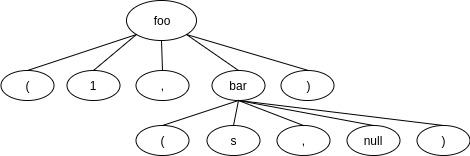
\includegraphics[width=0.5\textwidth]{AST}
  \caption{AST-дерево}
  \label{fig:AST-tree}
\end{figure}

\begin{figure}[H]
  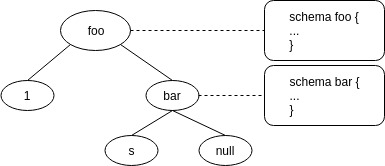
\includegraphics[width=0.5\textwidth]{call-tree}
  \caption{Дерево вызовов}
  \label{fig:call-tree}
\end{figure}

\begin{figure}[H]
  \schema{foo}
  {
    \es {1 == null} $\rightarrow$ \es{Throws IllegalArgumentException} \\

    \schema{bar}
    {
      \es{s is String} $\rightarrow$ \es{Returns (s + "1")} \\
      \es{s !is String} $\rightarrow$ \es{Returns (null)}
    }
    {
      \es{== null} $\rightarrow$ \es{Returns (Unit)}
    }
  }
  {}

  \caption{Дерево схем}
  \label{fig:schemas-tree}
\end{figure}

\begin{figure}[H]
  \schema{foo}
  {
    \es {1 == null} $\rightarrow$ \es{Throws IllegalArgumentException} \\

    \es{s is String && (s + "!") == null}  $\rightarrow$ \es{Returns (Unit)} \\

    \es{s !is String && null == null} $\rightarrow$ \es{Returns (Unit)}
  }
  {}

  \caption{Плоская схема}
  \label{fig:flat-schema}
\end{figure}

\begin{figure}[H]
  \schema{foo}
  {
    \es{s !is String} $\rightarrow$ \es{Returns (Unit)}
  }
  {}

  \caption{Сокращенная схема}
  \label{fig:reduced-schema}
\end{figure}

\begin{figure}[H]
  \es{s !is String}

  \caption{Результирующая информация}
  \label{fig:info-holder}
\end{figure}


\subsection{Применение системы эффектов в компиляторе Kotlin}

\subsubsection{Основы анализа потока данных}

Статический анализ в \lang{Kotlin} тесно связан с фреймворком анализа потока данных (англ. \eng{data-flow analysis}). Это довольно обширная и глубокая тема, и пересказать ее в рамках работы не представляется возможным. Тем не менее, нам необходимо обрисовать эту концепцию хотя бы в общих чертах, поскольку в противном случае разговор об улучшении анализа в \lang{Kotlin} будет слишком неконкретным.

Начнем с понятия графа потока управления (англ. \eng{control-flow graph, CFG}). Каждая инструкция в нем представлена одной вершиной, и если между вершинами $u$ и $v$ есть ребро, то это означает что после инструкции $u$ управление может быть передано
в инструкцию $v$.

Рассмотрим простой пример кода:

\begin{minted}{kotlin}
if (x == 0) {
    println("True branch")
} else {
    println("False branch")
}
println("If-end")
\end{minted}

Ему соответствует граф потока управления, как на рисунке \ref{control-flow-example}

\begin{figure}[h]
  \centering
  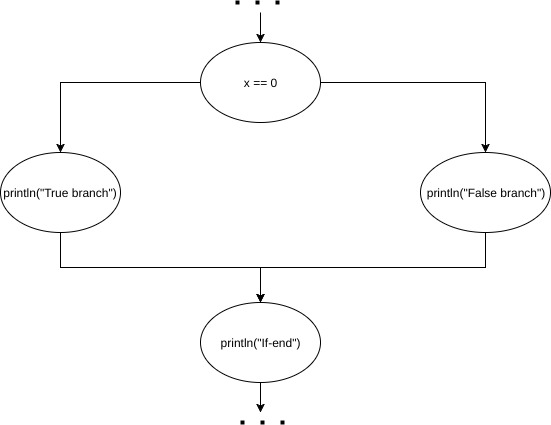
\includegraphics[scale=0.5]{img/control-flow-example}
  \caption{Пример графа потока управления}
  \label{control-flow-example}
\end{figure}


Так, после инструкции, вычисляющей условие в \code{if}, поток управления раздвоился, отражая тот факт, что мы не можем знать при статическом анализе (без дополнительных предположений), какая из веток выполнится. После ветки вновь сливаются в один поток, как и следовало ожидать.

Разумеется, граф потока управления не обязан быть ацикличным -- конструкции \code{for}, \code{while}, \code{goto} (безусловный переход) могут вносить в него обратные ребра.

Важно заметить, что любому возможному пути исполнения в программе обязательно соответствует некоторый путь в CFG, но обратное не верно. Например, путь может проходить через истинную ветку выражения \linebreak \code{if (x == 0) } и через истинную ветку выражения \code{if (x != 0)}, хотя между первым и вторым оператором могло и не быть никаких изменений переменной \code{x}, и иногда это даже можно доказать статически.
Тем не менее, это не нарушает консервативности анализа, поскольку при анализе будет обязательно рассмотрен любой реально возможный путь исполнения.

Конструкция графов потока управления сама по себе позволяет обнаружить совсем простые ошибки, вроде недостижимого кода из-за неправильного использования безусловных переходов. Однако она становится особо мощной и полезной, если использовать ее вместе с концепцией анализа потока данных.

\begin{definition}
  Анализ потока данных (англ. \eng{data-flow analysis})  -- это метод статического анализа, который основывается на извлечении информации из характеристик и свойств потока данных вдоль различных путей исполнения в программе.
\end{definition}

Основная идея основывается на наблюдении, что в любой момент времени при выполнении программы существует некоторое глобальное состояние, которое состоит из множества всех переменных, их значений, а также другой информации, зависящей от конкретного типа анализа (например, счетчик количества вызовов для функций, статус инициализации переменной, и т.д.). Тогда для каждой точки программы можно ввести понятие \term{значения потока данных} (от англ. \eng{data-flow value}), которое является абстракцией всех возможных глобальных состояний, которые можно наблюдать в данной точке. Для краткости, в дальнейшем мы будем писать DFV вместо <<значение потока данных>>.

В силу того, что потенциально количество возможных путей исполнения в программе может быть бесконечно \cite{dragon-book}, на практике делается два упрощения: во-первых, конкретное DFV не хранит историю, как управление могло придти к этой точке программы, а во-вторых, в зависимости от конкретного анализа, откидывается некоторая излишняя информация. Так, например, при анализе инициализации переменных, нам не важно, какие значения может иметь переменная, и на каких путях исполнения они могли быть получены. Достаточно знать, правда ли, что на любом пути исполнения, достигающем данную точку, данная переменная была инициализирована, или нет. Таким образом, для каждой переменной достаточно просто хранить бинарный флаг, что значительно упрощает реализацию на практике.

Мы не будем вдаваться в подробности того, как вычислять значения DFV, т.к. это выходит за рамки данной работы. Подробней про методы решения систем уравнений на поток данных можно прочитать в канонических источниках: \cite{dragon-book, muchnick}. В дальнейшем нам будет достаточно концепции графа потока управления и значения потока данных (DFV).

\subsubsection{Автоматическое приведение типов}

\label{section-upgrading-smartcasts}

Как мы уже говорили, \lang{Kotlin} поддерживает автоматические приведения переменной к более частному типу там, где это возможно. Чаще всего это возможно потому, что если управление дошло до определенной точки в программе, то должны выполняться некоторые ограничения на контекст.

Анализ умных приведений типов полностью основывается на анализе потока данных. Проблемы, описанные в главе 1, связаны с тем, что при извлечении из каждой инструкции начального DFV не учитываются межпроцедурные взаимодействия. Как раз здесь и может помочь система эффектов.

В качестве DFV для анализа умных приведений типов используется специальный класс \code{DataFlowInfo}, который хранит типовую информацию о переменных из контекста (обратите внимание на небольшую рассинхронизацию терминологии). Кроме того, данный класс поддерживает операции \code{or} и \code{and}, в точности соответствующие операциям, определенным нами в прошлом разделе для приближенных контекстов. Таким образом, этот класс естественно подходит на роль приближенного контекста.

Наконец, данный класс уже реализует всю необходимую логику для добавления и корректной обработки информации о подтипизации. 

В итоге, в данном пункте с точки зрения системы эффектов не требуется никакой дополнительной работы -- необходимо взять выражение и выполнить серию преобразований, описанных в предыдущем подразделе, используя \code{DataFlowInfo} в качестве приближенных контекстов. Фреймворк анализа потока данных сам обеспечит, чтобы полученная из системы эффектов информация была применена в нужном месте.


\subsubsection{Анализ инициализации переменных}

Анализ инициализации переменных также построен на основе анализа потока данных. Однако здесь для передачи информации из системы эффектов в компилятор нам понадобятся некоторые дополнительные усилия.

Для начала, вспомним, что проблемы с инициализацией появились из-за того, что у компилятора отсутствовала информация о том, что некоторые функции вызывают другие детерминированное число раз. Однако с точки зрения инициализации переменных, нас интересуют не точные счетчики вызовов каких-то процедур, а более общие понятия, которые мы будем называть \term{статусом вызовов}:

\begin{itemize}
  \item \code{UNKNOWN}, т.е. количество вызовов неизвестно

  \item \code{NOT INVOKED}, т.е. ровно ноль вызовов

  \item \code{EXACTLY ONCE}, т.е. ровно один вызов

  \item \code{AT LEAST ONCE}, т.е. по меньшей мере один вызов

  \item \code{AT MOST ONCE}, т.е. не более одного вызова
\end{itemize}

Таким образом, приближенный контекст для анализа инициализации переменных выглядит как отображение из функций в соответствующие им статусы вызовов. Преобразования \code{or} и \code{and} на статусах вызовов определяются довольно безыдейным перебором случаев. Их количество которых может быть несколько оптимизировано при более аккуратном подходе, но это в любом случае остается довольно технической работой, поэтому эти правила вынесены в приложение <TODO: INSERT APPENDIX REF HERE>.

Рассмотрим в качестве примера уже известный нам отрывок кода:

\begin{minted}{kotlin}
  val x: Int
  run {
    x = 42
  }
  println(x)
\end{minted}

Напомним, что изначально такой код не компилировался, поскольку компилятор считал переменную \code{x} в выражении \code{println(x)} не инициализированной. Это происходило из-за того, что для функции \code{run} не было гарантировано, что переданная в нее лямбда \code{ \{ x = 42\} } будет вызвана ровно один раз.

С точки зрения системы эффектов, для вызова функции \code{run} мы можем узнать, что переданная в нее лямбда была вызвана ровно один раз благодаря полученному статусу вызовов \code{EXACTLY ONCE}. Однако передать эту информацию в компилятор не так и просто.

Дело в том, что информация, необходимая для инициализации переменных, выражена в данном случае неявно (сравните это с автоматическим приведением типов, где информация о подтипизации была выражена явно). Если бы мы каким-то образом могли извлекать более явный эффект, например, \code{writes} (означающий, что функция пишет в некоторую переменную), то процесс интеграции был бы ничуть не сложней, чем в случае с приведениями типов.

Теоретически, можно было бы попытаться вывести этот эффект из тела лямбды, а затем аккуратно скомбинировать с эффектом \code{Calls}. Однако с точки зрения дизайна это является некоторым мошенничеством -- инициализация переменной на самом деле происходит в строке \code{x = 42}, в то время как мы приписываем инициализацию в строку вызова \code{run}. Из-за этого могут возникать чисто технические неприятности -- например, если \code{x} и так уже была инициализирована, то ошибка повторной инициализации будет выдана с неправильным номером строки.

Поэтому мы постараемся поступить более <<честно>> -- а именно, донести до компилятора информацию, что поток управления заходит в лямбду и затем выходит из нее, возвращаясь в точку вызова. Иными словами, мы бы хотели добавить ребро из инструкции вызова в начало декларации лямбды, а из конца декларации -- в следующую после вызова инструкцию (см. рисунок \ref{fig:flow-exactly-once-example})

\begin{figure}[h]
  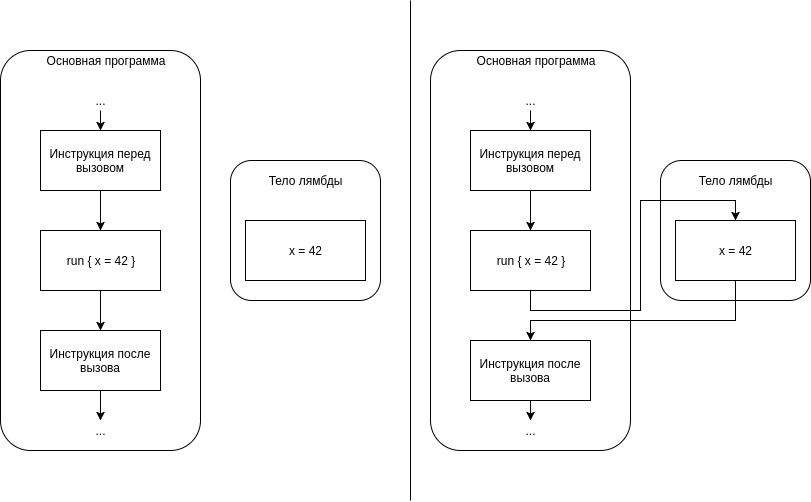
\includegraphics[width=\textwidth]{flow-exactly-once-example}

  \caption{Преобразование потока управления. \\ Слева -- исходная ситуация, справа -- после внесения изменений}
  \label{fig:flow-exactly-once-example}
\end{figure}

Этот подход, однако, значительно усложняется, если вместо лямбды используется именованная функция. Рассмотрим, например, следующий пример:

\begin{minted}{kotlin}
  val x: Int
  val block = { x = 42 }

  println(x)  // Not initialized yet
  run(block)
  println(x)  // Initialized once
  run(block)
  println(x)  // Re-initialization
\end{minted}

Именованную функцию можно вызывать несколько раз из различных участков кода -- и каждый вызов может иметь различное значение с точки зрения анализа инициализации. Например, в приведенном выше примере первый вызов корректно инициализирует переменную \code{x}, а вот второй вызов уже вызывает ошибку из-за повторной инициализации. Но поток управления в обоих случаях проходит по одной и той же инструкции, что может опять привести к проблемам с диагностическими сообщениями, и т.д.

В связи с этим, в рассматриваемой реализации было принято решение ограничиться рассмотрением только анонимных функций. Подчеркнем, что это не является недостатком разработанной системы, а, скорее, некоторыми техническими ограничениями предметной области, не позволяющими в полной мере воспользоваться информацией, поставляемой системой эффектов.

Кроме того, необходимо доставлять в компилятор информацию об \code{AT LEAST ONCE}, \code{NOT INVOKED} и \code{AT MOST ONCE}-вызовах. Первый наиболее актуален, т.к. подобные вызовы могут быть использованы для корректной инициализации \code{var}-переменных, допускающих повторное присваивание. Подробное описание того, как это можно сделать, в большей мере относится к анализу потока данных, нежели к системам эффектов, и потому выходит за рамки данной работы. Отметим, однако, что с точки зрения анализа потока данных, \code{AT LEAST ONCE} соответствует циклу \code{do-while} с условием, про которое не известно, сколько раз оно выполнится -- на этом наблюдении и основываются изменения, вносимые в поток управления.


\subsection{Реализация приведений типов в коллекциях}

Напомним, что изначально мы упоминали еще одну проблему, которую мы пока что никак не решили -- это автоматическое приведение типов в коллекциях, например в вызовах типа \code{ list.filter\{ x -> x is String \} }.

Мы не случайно отложили этот вопрос напоследок. Мы уже упоминали, что системы эффектов наиболее хорошо работают со свойствами функций, которые могут быть кратко выражены. Давайте аккуратно сформулируем, каково свойство вызова \code{filter}:

<<Вызов \code{filter} возвращает список, элементами которого являются те элементы исходного списка, на которых переданный предикат вернул \code{true} >>

Это довольно длинная мысль, и она никак не похожа на <<свойство функции, которое может быть выражено кратко>>. Если постараться записать это в более формальном синтаксисе, то можно неожиданно придти к теории множеств:

$$ S.filter(p) = \{ x \in S | p(x) \} $$

Эта запись говорит: \code{S.filter(p)} выдает множество $x$ из $S$ таких, что верен $p(x)$.

Таким образом, для задачи приведения типов в коллекциях лучше всего подходит формализм теории множеств, а не эффектов. Тем не менее, в данной работе мы покажем, как все-таки реализовать поддержку таких понятий в рамках системы эффектов. Помимо чисто научного интереса, это позволит лучше понять границы применимости системы эффектов и того, насколько сложно добавить в описанный фреймворк не очень свойственные ему понятия.

В дальнейшем мы будем использовать для примера функцию \code{filter}. Для упрощения мы будем рассматривать следующую ее сигнатуру:

\begin{minted}{kotlin}
  fun <T> filter(l: Collection<T>, p: (T) -> Boolean): List<T> {
    ...
  }
\end{minted}

\paragraph{Уточнение возвращаемого типа}

Начнем с того, что пока что в нашей системе нет вообще никакого способа сказать, что функция возвращает более конкретный тип, чем описанный в ее сигнатуре. Легче всего это сделать, если расширить семантику \code{Returns}, позволив ему возвращать не только значения, но и типы. Запись \code{Returns(T)} следует понимать следующим образом: функция возвращает \emph{неизвестное} значение типа $T$.

Заметим, что в предложенной в данной работе реализации по некоторым чисто техническим причинам был выбран другой путь, и был введен эффект \code{Hints(variable, type)}, который является полным налогом выражения \code{variable is type}. Их различие состоит в том, что \code{is} может появляться только слева от стрелки импликации, а \code{Hints} -- только справа. В дальнейшем мы будем пользоваться синтаксисом с перегруженным \code{Returns}, дабы не плодить излишние сущности.

Таким образом, мы уже можем написать часть схемы для \code{filter}, которая выглядит следующим образом:

\schema{filter(l, p)}
{
  \es{true} $\rightarrow$ \es{Returns ( List < ... > )} \\
}{}

Теперь наша задача состоит в том, чтобы вместо многоточия вставить тип, определяемый поведением лямбды, т.е. тип аргумента лямбды, при условии, что предикат вернул \code{true}.


\paragraph{Оператор at.}

Пусть у нас имеется схема эффектов для предиката \code{p}. Нам необходимо как-то выразить ту мысль, что нас будет интересовать только та часть схемы, которая соответствует случаю, когда предикат вернул \code{true}. Если внимательно посмотреть на эту формулировку, то можно заметить, что она  \emph{в точности повторяет операцию фильтрации схемы}, которую мы определили в пункте \ref{section-back-inference}.

Таким образом, нам нужно просто предоставить пользователем возможность пользоваться операцией, которая до этого была внутренней для системы эффектов. Для этого мы вводим бинарный оператор \code{at}. Выражение \code{S at E}, где \code{S} -- схема, a \code{E} -- эффект, возвращает схему, соответствующую схеме \code{S} отфильтрованной по эффекту \code{E} как было определено в пункте \ref{section-back-inference}.

Теперь мы можем еще на шаг продвинуться к спецификации \code{filter}:

\schema{filter(l, p)}
{
  \es{true} $\rightarrow$ \es{Returns ( List < p at Returns(true) ... > )}
}{}


\paragraph{Оператор typeOf.}

Теперь вместо многоточия осталось вставить конструкцию, которая бы корректно вывела тип, который имеет аргумент лямбды в схеме \code{p at Returns(true)}.

Однако перед тем, как ввести эту операцию, остановимся на одним маленьком нюансе, на котором мы не заострили внимание в прошлом параграфе. Дело в том, что в момент аннотации \code{filter}, невозможно знать, какое имя будет у аргумента лямбды, поскольку объявление лямбды будет написано в месте вызова \code{filter}. Следовательно, мы не можем сослаться на этот аргумент.

Если для сравнения посмотреть на спецификацию \code{filter} в терминах теории множеств, то там \emph{вводится} новая переменная $x$ с помощью конструкции $\{ x \in S | P(x) \}$. Мы могли бы поступить по аналогии, и сделать еще одну новую конструкцию для введения переменных -- нечто в духе \code{let x in ...}, навеянное языками семейства ML.

Однако в приведенной реализации удалось этого избежать благодаря тому, что синтаксис \lang{Kotlin} позволяет в сигнатуре функции указать именовать аргументы принимаемых на вход лямбд:

\begin{minted}{kotlin}
  fun <T> filter(s: Collection<T>, p: (arg: T) -> Boolean): List<T> {
    ...
  }
\end{minted}

Теперь мы можем ввести оператор \code{typeOf}. Выражение \code{S typeOf V}, где \code{S} -- схема, а \code{V} -- переменная, выдает тип, подтипом которого гарантированно является \code{V} в схеме \code{S}, и из таких наиболее частный. Другими словами, оператор \code{typeOf} в точности соответствует оператору слияния из пункта \ref{section-back-inference}, использующему в качестве приближенных контекстов классы \code{DataFlowValue} из анализа приведений типов в пункте \ref{section-upgrading-smartcasts}.

Таким образом, полная спецификация \code{filter} выглядит следующим образом:

\schema{filter(l, p)}
{
  \es{true} $\rightarrow$ \es{Returns ( List <(p at Returns(true)) typeOf arg> )}
}{}

В ней, однако, существует одна досадная, чисто техническая неточность. Дело в том, что при конкретном вызове \code{filter} вместо \code{p} будет подставлена лямбда. Эта лямбда может иметь другое мнение на счет того, как должен называться ее первый параметр -- соответственно, и ее схема эффектов будет использовать другое имя для этого параметра. Например, вызов \code{filter(S, \{ x -> x is String \})}, как можно видеть, использует для первого аргумента имя \code{x}, в то время как с точки зрения схемы этот же самый первый аргумент имеет имя \code{arg}

В связи с этим, нам необходимо выполнить композицию подстановок -- сначала нужно подставить в схему эффектов \code{filter} все параметры вызова, а затем в тела лямбд нужно подставить корректные аргументы. Для того, чтобы было проще понять, в какие лямбды нужно подставить какое имя, можно более явно специфицировать вызов, и вместо \code{p at ...} писать \code{p(arg) at ...}.

Таким образом, конечный синтаксис записис эффектов для \code{filter} выглядит следующим образом:

\schema{filter(l, p)}
{
  \es{true} $\rightarrow$  \es{Returns ( List <(p(arg) at Returns(true)) typeOf arg> )}
}
{}

\paragraph{Анализ.}
Как можно видеть, синтаксис получился не из самых приятных. Кроме того, поддержка подобных функций потребовала значительных усилий со стороны системы эффектов -- пришлось ввести несколько новых конструкций, расширить грамматику. В оправдание можно сказать, что эти конструкции не были полностью новыми -- они уже использовались внутри системы, и нужно было только выдать им соответствующие операторы в грамматике. Тем не менее, количество усилий определенно выше, чем для того же \code{Calls}. Почему же так вышло? Не получили ли мы негибкую систему, которая способна формализовать лишь узкий, заранее предопределенный круг понятий?

Ответ состоит в том, что разработанная система эффектов, несмотря на введенные расширения, все же остается системой \emph{эффектов}. Мысль, которую мы пытались формализовать в спецификации \code{filter}, интуитивно противоречит пониманию эффекта -- по сути, она является спецификацией того, как работает \code{filter}, а не некоторым <<побочным>> эффектом вычисления. 

С другой же стороны, эффект \code{Calls} превосходно укладывается в эту концепцию -- соответственно, и его добавление в систему не потребовало вообще никаких дополнительных действий. К примеру, таким же свойством обладают <<классические>> эффекты \code{read} и \code{write}, часто рассматриваемые в статьях и работах по системам эффектов -- их добавление также не потребует практически никаких усилий от системы эффектов (однако могут возникнуть довольно нетривиальные задачи при \emph{использовании} информации об этих эффектах).

В этом, вобщем-то, нет ничего удивительного -- чем больше понятий способна формализовать та или иная логическая система, тем более она сложна и тем больше в ней конструкций. Мы изначально отказались от мощных, но сложных систем, реализованных в виде формальных языков спецификаций -- как следствие, добавление новых понятий обошлось относительно дорого.

Мы видели, что с точки зрения синтаксиса, теория множеств позволяет формализовать это утверждение ощутимо короче и намного ясней. Однако введение теории множеств \emph{только} для формализации контракта \code{filter} и других функций, работающих с коллекциями, выглядит неоправданным с практической точки зрения -- это серьезный пласт новых понятий, терминов, синтаксиса и работы по реализации всего этого на практике. 

В связи с этим, в реализации, приложенной к данной работе, было принято решение остановиться на решении проблемы умных приведений типов в коллекциях с помощью системы эффектов.